\documentclass{article}

\usepackage{amssymb}
\usepackage{graphicx} 
\usepackage{graphics}
\graphicspath{{figures/}} 

\usepackage{hyperref}
\hypersetup{
    colorlinks=true,
    linkcolor=blue,
    filecolor=magenta,      
    urlcolor=cyan,
}
\usepackage{listings}
\usepackage{color}

\definecolor{dkgreen}{rgb}{0,0.6,0}
\definecolor{gray}{rgb}{0.5,0.5,0.5}
\definecolor{mauve}{rgb}{0.58,0,0.82}

\lstset{frame=tb,
  language=Java,
  aboveskip=3mm,
  belowskip=1mm,
  showstringspaces=false,
  columns=flexible,
  basicstyle={\small\ttfamily},
  numbers=none,
  numberstyle=\tiny\color{gray},
  keywordstyle=\color{blue},
  commentstyle=\color{dkgreen},
  stringstyle=\color{mauve},
  breaklines=true,
  breakatwhitespace=true,
  tabsize=3
}



\begin{document}
\title{Pyshifts User Guide}
\author{Jingru Xie}
\maketitle


\tableofcontents


\newpage
\section{Introduction}
\subsection{Overview}

PyShifts is a PyMol based graphical analysis tool that utilize chemical shifts to assess the global quality of NMR structures of RNA. Pyshifts takes structure and measured chemical shifts file as input, using various predictors to predict chemical shifts for the structure (or different states in an ensemble if input is an ensemble), comparing it to measured chemical shifts, analyze and visualize difference. Or, it can take external predicted chemical shifts, comparing it to measured chemical shifts and visualize difference. 

Codes and resources are freely available at \href{https://github.com/atfrank/PyShifts}{out github site}. For more information on theoretical basis as well as our promising test results, see \href{http://linktoManuscript}{manuscript}. 

Pyshifts is tested on Mac OS X El Captain, the following manual uses Mac OS X as example. 

\subsection{Copyright Notice}

The PyMOL Plugin source code is copyrighted, but you can freely use and copy it as long as you don't change or remove any of the copyright notices.

This PyMOL Plugin is Copyright\textcopyright 2016 by Jingru Xie (\href{mailto:jingrux@umich.edu}{jingrux@umich.edu}) and Aaron T. Frank (\href{mailto:afrankz@umich.edu}{afrankz@umich.edu}).
                          
 All Rights Reserved.



\newpage
\section{Installation}
\subsection{Requirements}
Pyshifts is a plugin in PyMOL, an open source Python-enhanced molecular graphics tool. Python of version 2.7.10 and PyMOL are REQUIRED for Pyshifts.


\subsection{Installation guide}
\begin{enumerate}
\item{Python}

Python version of 2.7.10 (and 2.7.10 only), which is freely available at \url{https://www.python.org/downloads/release/python-2710/}.

If your current Python version is not 2.7.10, and you prefer not to change it, you can use the following commands to create a Python 2.7.10 environment temporarily for Pyshifts:

\begin{lstlisting}
conda create -n pyshifts python=2.7.10
source active pyshifts
\end{lstlisting}
After each use of Pyshifts, use
\begin{lstlisting}
source deactivate pyshifts
\end{lstlisting}
to go back to your normal Python settings.
\item{PyMOL}

You can obtain PYMOL at sourceforge https://sourceforge.net/projects/pymol/.

\item{Adding Pyshifts to PyMOL}

Download or clone this git repository.
Open PyMOL and then go to "Plugin"$\to$"Plugin manager"$\to$"Install new plugin", and choose the Pyshifts.py file in your local Pyshifts repository. For this step PyMOL need to be run with the Tcl/Tk interface, read more on PyMOL wiki \url{https://pymolwiki.org/index.php/Plugins}.

\end{enumerate}



\newpage
\section{Getting started with Pyshifts}

\subsection{Layout}

Once you have Pyshifts successfully installed in PyMOL, you can see it under "Plugin" menubar. Click to run.

\begin{figure}[htbp]
\centering
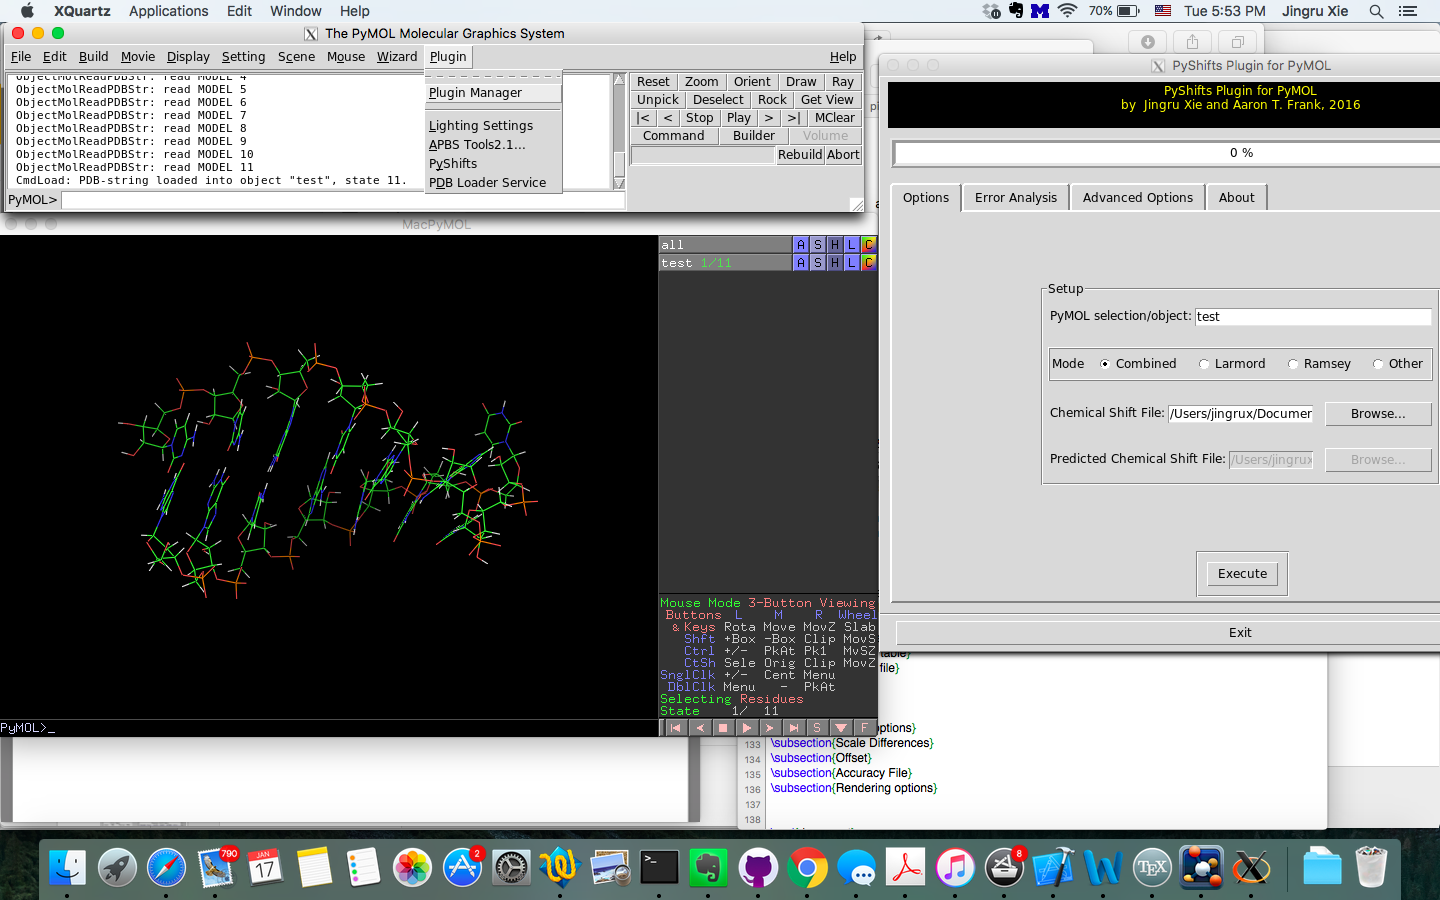
\includegraphics[width=0.7\textwidth]{layout_0.png}
\caption{Run Pyshifts from PyMOL.}
\label{fig:layout0}
\end{figure}


A new window will pop up. This is the main page of Pyshifts. Basic options will show in main page. At the top of the window is a progress bar. When running, progress bar will show the progress of your current operation. Under progress bar is the main menu bar. By clicking on those tabs you can switch back and forth among the four tabs: "Options" (default), "Error Analysis", "Advanced Options" and "About".

\begin{figure}[htbp]
\centering
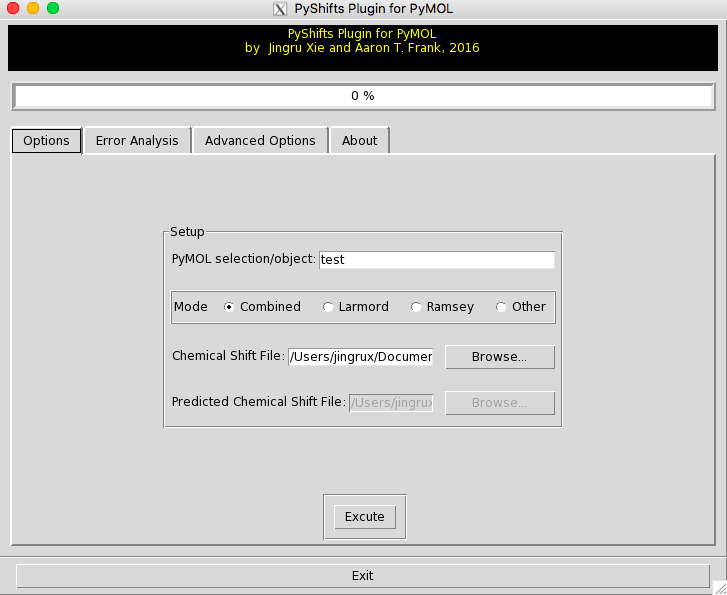
\includegraphics[width=0.6\textwidth]{main}
\caption{Pyshifts default window.}
\label{fig:layout1}
\end{figure}



\subsection{Global parameter}
Pyshifts use LarmorD as one of its predictor. Before we start working on test case, first you have to set file path to LarmorD parameters correctly. To do this, create a file "pymolrc" under your root folder
\begin{lstlisting}
vi ~/.pymolrc
\end{lstlisting}
Under insert mode, add a line to that file
\begin{lstlisting}
cd /Users/jingrux/Documents/GitSoftware/Pyshifts
\end{lstlisting}


\subsection{Test case}
To start with, let's first have a try on our test case. Test case is an NMR solution structure of a 14-mer hairpin RNA with cUUCGg tetraloop \href{http://www.rcsb.org/pdb/explore.do?structureId=2koc}{PDB: 2KOC}. The structure coordinates (2KOC\_test.pdb), reference chemical shifts (measured\_shifts\_2KOC.dat) and an example predicted chemical shifts file (predicted\_shifts\_2KOC.dat) are all included in "test" folder which comes with the original package. Or you can always download the "test" folder from github site \url{https://github.com/atfrank/PyShifts}.

First, load structure into PyMOL as "test". In PyMOL command line, type in
\begin{lstlisting}
load test/2KOC_test.pdb, test
\end{lstlisting}

A structure will show in PyMOL window. This is frame of 2KOC, our test case.
\begin{figure}[htbp]
\centering
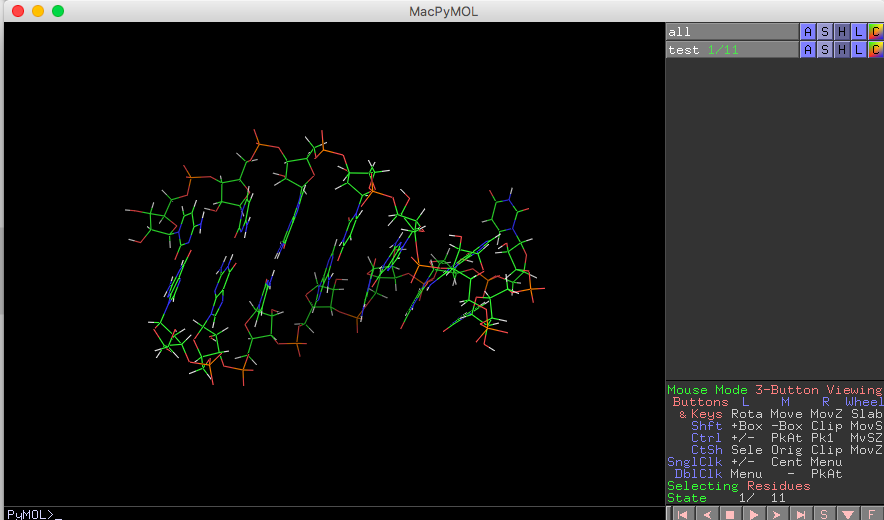
\includegraphics[width=0.7\textwidth]{test_ensemble}
\caption{Test ensemble in PyMOL.}
\label{fig:test1}
\end{figure}

In Pyshifts window, find the corresponding file and enter in "Chemical Shifts File" entry. The measured chemical shifts for 2KOC is provided as measured\_shifts\_2KOC.dat in "test" folder. 
\begin{figure}[htbp]
\centering
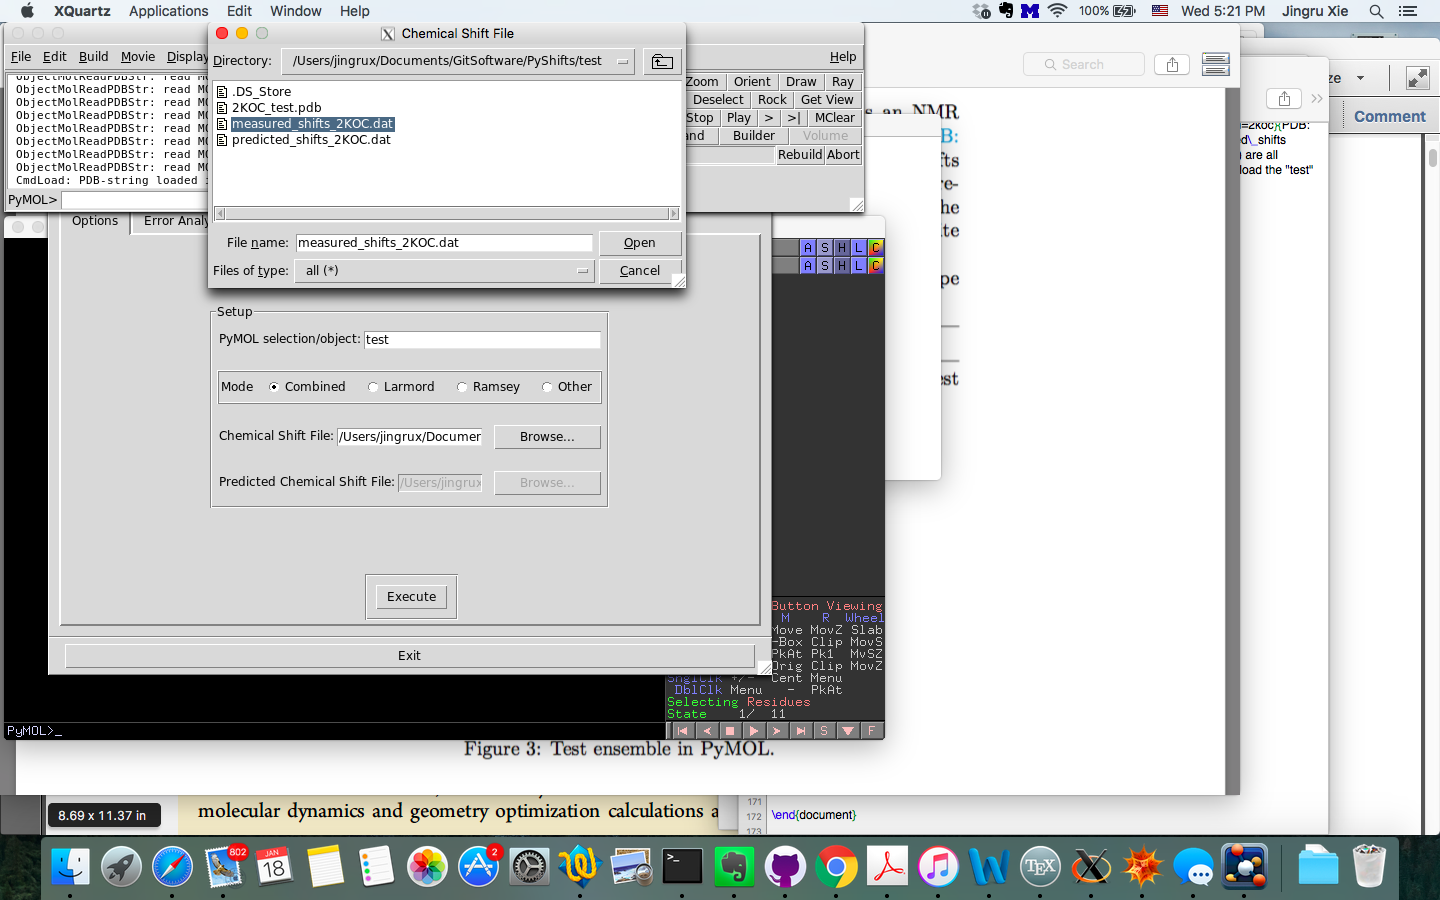
\includegraphics[width=0.7\textwidth]{test2}
\caption{Test measured chemical shifts file}
\label{fig:test2}
\end{figure}

Click on 'execute' button. It may take some time for Pyshifts to complete computing.The progress bar will show your progress in percentage.

Then go to "Error Analysis" tab, click on "Compare shifts". Error Table on the left will be filled with state number and their corresponding MAE (mean absolute error), Pearson coefficient, RMSE (Root mean square error). We will talk about it later in "Error Analysis" section. The table is by default sorted in MAE ascending order.

At the meantime the first few states on top of error table will show in PyMOL. Error for each residues are shown in spheres of different size and color. 

 
\begin{figure}[htbp]
\centering
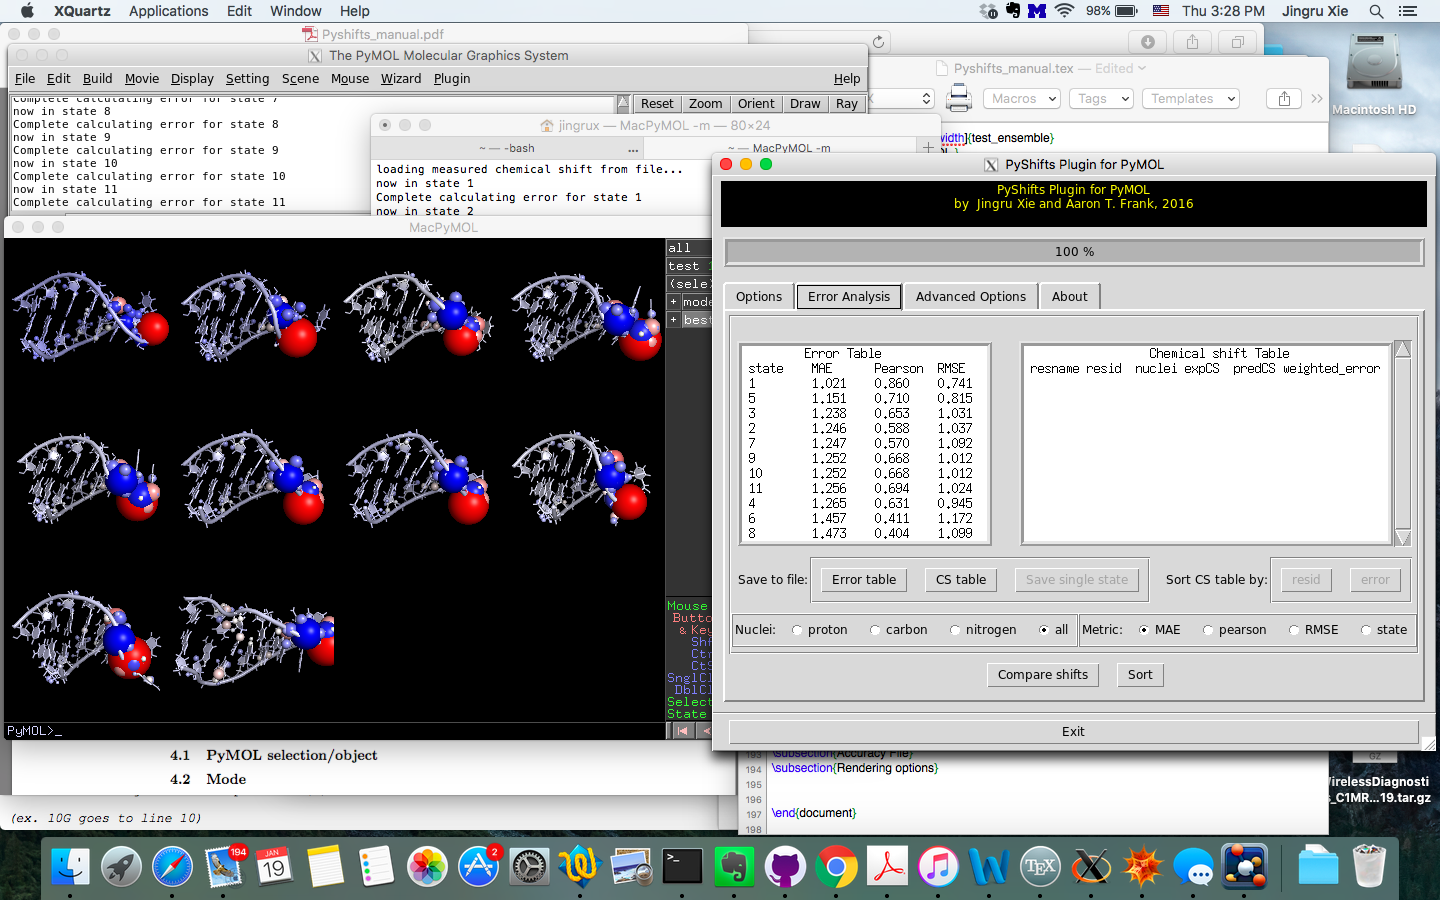
\includegraphics[width=0.7\textwidth]{test3}
\caption{Test error analysis overview}
\label{fig:test3}
\end{figure}
 
Then double click on one of the state in "Error Table", "Chemical shift Table" will be filled with all the individual residue in your selected state. Each residual is specified by residue name (resname), residue id (resid), nuclei, experimental chemical shifts (expCS) given by the reference file, predicted chemical shifts (predCS) given by built-in predictor, and weighted error (weighted\_error) between them.

\begin{figure}[htbp]
\centering
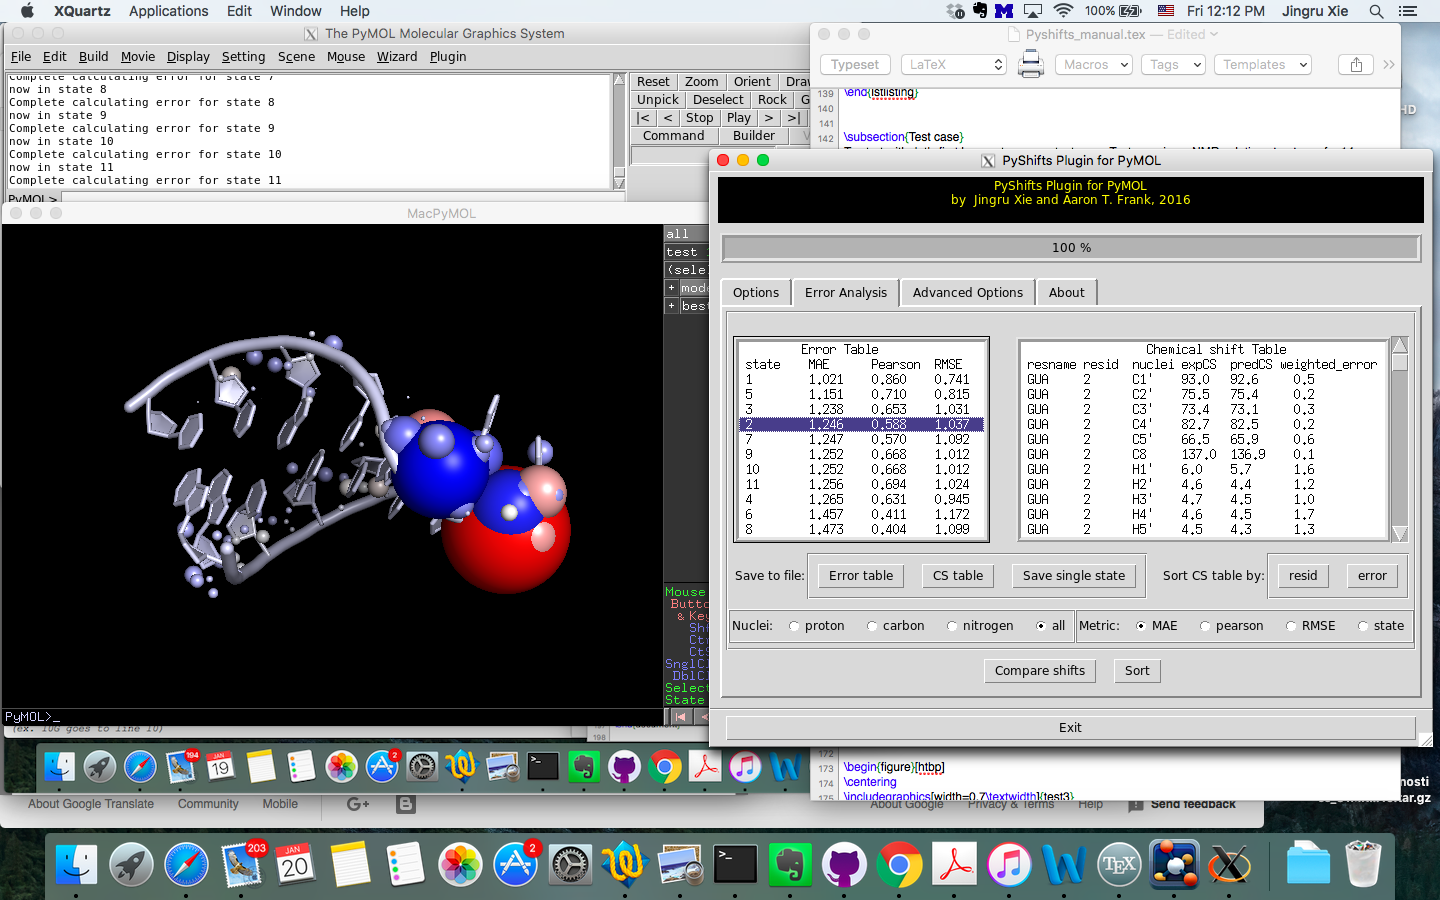
\includegraphics[width=0.7\textwidth]{test4}
\caption{Test Chemical shift table and a single state in PyMOL}
\label{fig:test4}
\end{figure}

At the meantime the state you chose will be enlarged in PyMOL window, showing details of that state.

If you double click on one row in chemical shift, that specific residual will also be highlighted in PyMOL.

In the following three sections, detailed configuration and usage will be introduced.
\newpage
\section{Options (Setup)}

\subsection{PyMOL selection/object}
PyMOL selection/object should be a valid name of a Pymol object that has been loaded. For example if you load a 2LPS.pdb file into PyMOL and name the object as "batman", then you should use "batman" in PyMOL selection/object entry (rather than 2LPS).
 
\subsection{Mode}
\subsubsection{Using predictor}
Pyshifts provided you with two predictors and three modes: LarmorD, Ramsey or a combination of them. By default Pyshifts use combined mode to realize a high accuracy of prediction. In this mode, both LarmorD and Ramsey are used for prediction, and an average of them will be taken for analysis.

In each of the three modes, only one chemical shifts file is needed. The bottom line "Predicted Chemical Shift File" will be disabled.
\subsubsection{Using external predicted chemical shifts file}
The last mode in Mode selection, "Other" is somehow different from all other modes. In this mode, Pyshifts will not run predictor, rather, it will use the predicted chemical shifts data you provided. 

In this mode, two chemical shifts files should be provided: one measured chemical shifts, one set of chemical shifts for all states as reference, same as before; and another predicted measured chemical shifts file, which contains the predicted chemical shifts for each residue in each mode. The bottom line "Predicted Chemical Shift File" will be put into use.

An example predicted chemical shifts file for 2KOC is also given in "test" folder. You can play around with "Other" mode in our test case using this file.

\newpage
\section{Error Analysis}
\subsection{Error Table}
Error Table shows the difference between measured predicted chemical shifts of each state based on three metrics: MAE, Pearson matrix coefficient and RMSE. For a structure with $N$ nuclei, MAE and RMSE are computed as follows:
$$MAE = \frac{1}{N}\sum_{n=1}^{N} |measuredCS[i]-predictedCS[i]|$$
$$RMSE = \frac{1}{N}\sum_{n=1}^{N} (measuredCS[i]-predictedCS[i])^2$$
Where $measredCS[i]$ ($predictedCS[i]$) denotes measured (predicted) chemical shift for the $ith$ nucleus.
Pearson coefficient is computed using Python function $scipy.stats.pearsonr$.

By default the summation goes over all kinds of nuclei in the structure (provided that nucleus has chemical shifts data given). You can also make Pyshifts only calculate the error of either carbons, hydrogens or nitrogens. This can be achieved using Nuclei selection.

\subsubsection{Sort table: Nuclei and Metric}
Error table can be sorted based on a combination of different nuclei and metric by changing selections in the lower row.
\begin{figure}[htbp]
\centering
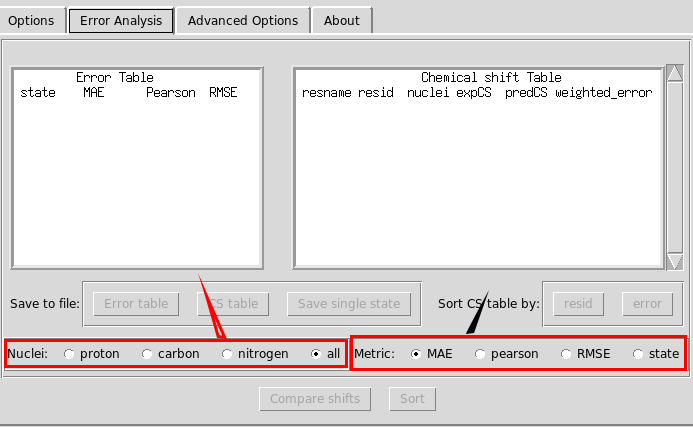
\includegraphics[width=0.7\textwidth]{sort_error_table_copy}
\caption{Sort error table based on different nuclei and metrics}
\label{fig:error_analysis_1}
\end{figure}
When Nuclei selection in selections other than "all", only selected group of residues will be used to calculate error and only shown in chemical shift table and Pymol.

Note after you change your selection of nuclei or metric, use "sort" button to realize change.

\subsection{Chemical Shifts Table}
Chemical shifts (both predicted and measured) and "weighted erorr" are displayed in chemical shifts table for each individual nuclei in your selected state. 

Weighted error is calculated based on the difference between predicted and measured chemical shifts and predictor accuracy:
$$weighted_error[i] = \frac{predictedCS-measuredCS}{accuracy[i]}$$
Predictor accuracy can be customized by providing an accuracy file, or you can choose not to weight the errors in advanced options. (See next chapter)
\subsubsection{Sort table}
Chemical shift Table can be sorted by residue id ascended or in error descending order.

\subsection{Save to file}
Both error table and chemical shift table can be saved to a .dat file. Tables should have been filled in Pyshifts before they can be saved. If you only want to save the chemical shifts data of your selected state, use "Save single state".


\newpage
\section{Advanced options}
\subsection{Scale Differences}
Predictor yield different errors for different nuclei. "Scale Differences" take predictor error into account. When in "Yes", errors used for analysis will be weighted error (absolute error divided by weight, which is given as accuracy file, or default setting in code).
\subsection{Offset}
"Offset" option can shift the error of a certain kind of nuclei, to account for chemical shifts offset that always exist in NMR measurements.
\subsection{Accuracy File}
Optional. Weight used to scale difference is given in accuracy file. When not given, a default LarmorD accuracy list will be used. 
\subsection{Rendering options}
\begin{enumerate}
\item{Colors}

Colors used to render error spheres in Pymol. Default setting is "blue\_white\_red", which will show negative error as blue, positive as red, while zero error is white.
\item{Sphere size}

A scale of how large the error sphere will show in Pymol. Depending on the weighted error of you specific case, this option should be adjusted to give the best visualizing performance. Default setting is $0.4$.
\item{No. models to display}

Number of models to display. How many models to display in Pymol after each Comparing shifts and sorting behavior. Default is 10.
\end{enumerate}



\end{document}